\documentclass[11pt]{article}
\usepackage[margin=1in]{geometry}
\usepackage{amsmath,amssymb,amsthm}
\usepackage{algorithm}
\usepackage{algpseudocode}
\usepackage{booktabs}
\usepackage{hyperref}
\usepackage{tikz}
\usepackage{xcolor}
\usetikzlibrary{arrows.meta,positioning,fit,backgrounds,shapes.geometric,calc}

\newtheorem{definition}{Definition}
\newtheorem{theorem}{Theorem}
\newtheorem{proposition}{Proposition}
\newtheorem{example}{Example}

\title{Tighter Approximation Schemes for\\Chain-Graph Logical Credal Networks}
\author{IBM Research}
\date{}

\begin{document}
\maketitle

\begin{abstract}
A chain-graph Logical Credal Network (LCN) admits a factorization that captures its
Local Markov Condition (LMC) independence assumptions. The current \texttt{cn/} pipeline
exploits this by compiling the LCN into a \emph{credal network}: a directed graph whose
local credal sets $K(\mathrm{child}\mid\mathrm{parents})$ are interval-valued and computed
per family, then performing posterior inference (Credal Variable Elimination) over the
\emph{strong extension} of that credal network. The strong extension is generally a
\emph{proper superset} of the LCN's distribution set, so the computed posterior marginal
bounds are looser than the exact LCN bounds. This note dissects the two distinct sources
of this looseness on a running example (the \texttt{alarm} network), proposes five
approximation schemes that produce tighter outer approximations---hence tighter posterior
bounds---illustrates each on the example, explains how the existing inference algorithms
(Credal VE, Interval BP, ApproxLP, Credal CTE, Credal IJGP) all inherit the tightening,
and gives a validation strategy based on certified local solves and the existing LMC
factorization verifier.
\end{abstract}

\section{Background and notation}

Let an LCN over propositional atoms $\mathbf{V}=\{V_1,\dots,V_n\}$ define a set of joint
distributions
\[
  \mathcal{D}_{\mathrm{LCN}} \;=\; \bigl\{\, P \in \Delta(2^{\mathbf{V}}) \;:\; P \text{ satisfies every sentence } s \,\bigr\},
\]
where each sentence $s$ is a Type-1 constraint $\ell \le P(\varphi) \le u$ or a Type-2
constraint $\ell \le P(\varphi\mid\psi) \le u$. When the LCN's structure graph is a chain
graph, the joint factorizes over the families (child $+$ parents) of the simplified
structure graph,
\begin{equation}\label{eq:factor}
  P(\mathbf{V}) \;=\; \prod_{v} P\!\bigl(\mathrm{ch}_v \mid \mathrm{pa}_v\bigr),
\end{equation}
and this factorization reproduces exactly the LMC independencies
(cf.\ \texttt{docs/ISIPTA2025\_LCNs.pdf} Sec.~3, \texttt{docs/LCN\_IJAR\_Revised.pdf}).

The \texttt{cn/} pipeline realizes \eqref{eq:factor} in three stages, each of which is
implemented in a distinct module:
\begin{enumerate}
  \item \textbf{Symbolic factorization} (\texttt{cn/factorization.py}): enumerate the
    families and record, per family, the child, parents, flattened atom scope and the
    LCN sentences \emph{attached} to that family.
  \item \textbf{Local credal sets} (\texttt{cn/local\_credal\_sets.py}): for each family
    and each interpretation of its scope, solve a (fractional) optimization problem to
    obtain the lower/upper bound $[\underline{p},\overline{p}]$ of the conditional
    $P(\mathrm{ch}_v=c \mid \mathrm{pa}_v=\pi)$. The method axis carries exactly two
    settings (Section~\ref{sec:api}): \texttt{method="linear"} (the baseline) treats each
    family \emph{in isolation}, and \texttt{method="linear-tight"} solves the same family
    against every in-scope LCN sentence plus the scope-restricted LMC equalities (scheme
    D1 of Section~\ref{sec:designs}).
  \item \textbf{Inference over the strong extension} (\texttt{cn/vertices.py},
    \texttt{cn/cve.py}): enumerate the extreme points of each local credal set and run
    Credal Variable Elimination, which optimizes over the strong extension---each local
    credal set, for each parent configuration, contributes a freely and independently
    chosen extreme point.
\end{enumerate}

\subsection{Build API: two methods, two orthogonal knobs}\label{sec:api}

The schemes below are exposed through the existing build entry points
(\texttt{CredalNetwork.from\_lcn}, \texttt{CredalNetworkVertices.from\_lcn}) without
multiplying flags. The previous \texttt{method="nlp"} option (which added only
\emph{pairwise} parent marginal independence) is \textbf{removed}: it is a strict
half-measure for source~A, dominated by D1 below, and its bilinear program added solver
fragility for little tightening. The surface is therefore:
\begin{itemize}
  \item \texttt{method} $\in\{$\texttt{"linear"}, \texttt{"linear-tight"}$\}$. \texttt{"linear"}
    is today's per-family-in-isolation baseline (unchanged). \texttt{"linear-tight"} is
    scheme~D1: each family is solved against every LCN sentence whose atom scope lies inside
    the family scope, plus the scope-restricted LMC bilinear equalities.
  \item \texttt{solver} $\in\{$\texttt{"ipopt"}, \texttt{"scip"}$\}$ (already present). On
    \texttt{"linear-tight"}, \texttt{solver="scip"} \emph{is} scheme~D3: it solves the
    enriched local program to certified global optimality; \texttt{"ipopt"} is the fast,
    hardened (multi-restart $+$ SLSQP-fallback) variant of the same program.
  \item \texttt{merge\_budget} $k$ (new): scheme~D2. A pre-factorization pass merges adjacent
    families whose combined scope is $\le k$ before \texttt{ChainGraphFactorization.build};
    $k{=}1$ is no merge (today), $k{=}$ full scope is exact. Orthogonal to \texttt{method}
    and \texttt{solver}.
\end{itemize}
Thus D1 is the \emph{core} of \texttt{"linear-tight"}, while D2 ($k$) and D3 (\texttt{solver})
are independent cost-vs-tightness dials rather than separate method names. (This \texttt{cn/}
factorization \texttt{method} is unrelated to the identically named parameters of
\texttt{ibp.py} and \texttt{map/exact\_map.py}.)

\section{Running example: the \texttt{alarm} network}\label{sec:example}

We use \texttt{examples/alarm.lcn} throughout. It has five atoms $\{A,B,C,D,E\}$ and five
sentences:
\begin{verbatim}
  s1: 0.1  <= P(B)               <= 0.2
  s2: 0.05 <= P(E)               <= 0.1
  s3: 0.6  <= P(A | (B or E))    <= 0.9
  s4: 0.5  <= P(not(C xor D) | A) <= 0.7   ; True
  s5: 0.05 <= P(A)               <= 0.1
\end{verbatim}
Its structure is a chain graph. The simplified structure graph has the compound node
$C\!-\!D$ (because $s4$ ties $C$ and $D$ together through $C \oplus D$), so the families
and the LMC independencies the pipeline derives are:
\begin{center}
\begin{tabular}{lll}
  \toprule
  Family & Attached sentences & \\
  \midrule
  $P(A \mid B,E)$   & $s1,s2,s3,s5$ & \\
  $P(B)$            & $s1$ & \\
  $P(E)$            & $s2$ & \\
  $P(C\!-\!D \mid A)$ & $s4,s5$ & \\
  \bottomrule
\end{tabular}
\qquad
\begin{tabular}{l}
  \toprule
  LMC independencies \\
  \midrule
  $(B \perp E)$ \\
  $(C \perp B,E \mid D,A)$ \\
  $(D \perp B,E \mid C,A)$ \\
  \bottomrule
\end{tabular}
\end{center}
The factorization is $P(A\mid B,E)\,P(C\!-\!D\mid A)\,P(B)\,P(E)$.

\paragraph{Local credal sets computed today (\texttt{method="linear"}).}
Solving each family in isolation gives the conditionals below (lower/upper, rounded). Note
the many vacuous $[0,1]$ entries---these are exactly where gap A bites.
\begin{center}
\begin{tabular}{llcll}
  \toprule
  \multicolumn{2}{l}{$P(A\mid B,E)$} & & \multicolumn{2}{l}{$P(C\!-\!D\mid A)$} \\
  \cmidrule(r){1-2}\cmidrule(l){4-5}
  $A{=}0,B{=}0,E{=}0$ & $[0.956,\,1.0]$   & & $C{=}0,D{=}0,A{=}1$ & $[0,\,0.7]$ \\
  $A{=}1,B{=}0,E{=}0$ & $[0,\,0.044]$     & & $C{=}0,D{=}1,A{=}1$ & $[0,\,0.5]$ \\
  $A{=}0,B{=}0,E{=}1$ & $[0,\,1.0]$       & & $C{=}1,D{=}0,A{=}1$ & $[0,\,0.5]$ \\
  $A{=}1,B{=}0,E{=}1$ & $[0,\,1.0]$       & & $C{=}1,D{=}1,A{=}1$ & $[0,\,0.7]$ \\
  $\cdots$ (rows with $B{=}1$ or $E{=}1$) & $[0,\,1.0]$ & & $\cdots$ ($A{=}0$ rows) & $[0,\,1.0]$ \\
  \bottomrule
\end{tabular}
\end{center}
Two phenomena stand out and recur in the discussion below:
\begin{itemize}
  \item \textbf{$s3$ only constrains the $(B\!\lor\!E)$ corner.} $s3$ bounds
    $P(A\mid B\lor E)$, i.e.\ the conditional given the \emph{disjunction}. It says nothing
    directly about $P(A\mid B{=}0,E{=}1)$ or $P(A\mid B{=}1,E{=}0)$ individually, so those
    parent configurations come back vacuous $[0,1]$---even though, jointly with $s5$
    ($P(A)\in[0.05,0.1]$) and the marginals $s1,s2$, the LCN pins them far tighter.
  \item \textbf{$s4$ constrains a sum, not a single state.} $s4$ bounds
    $P(\lnot(C\oplus D)\mid A){=}P(C{=}D\mid A)$, i.e.\ the sum of the two diagonal states
    $P(C{=}0,D{=}0\mid A)+P(C{=}1,D{=}1\mid A)$. The isolated family LP can therefore push
    any single state to its extreme (hence $[0,0.7]$ / $[0,0.5]$), and for $A{=}0$ there is
    no constraint at all, giving $[0,1]$.
\end{itemize}
This is the concrete object the schemes of Section~\ref{sec:designs} tighten.

\section{Two sources of looseness}\label{sec:sources}

Write $\widetilde{\mathcal{D}}$ for the joint credal set actually optimized by CVE. We
have $\mathcal{D}_{\mathrm{LCN}} \subseteq \widetilde{\mathcal{D}}$, and the inclusion is
typically strict for \emph{two independent reasons}.

\subsection{(A) Local-set widening}

For family $v$ the pipeline computes
\[
  K_v^{\mathrm{local}}
  = \Bigl\{\, P(\mathrm{ch}_v\mid\mathrm{pa}_v) \;:\; \text{the sentences \emph{attached to family }} v \text{ hold} \Bigr\},
\]
because \texttt{\_linear\_rows\_and\_obj} loads only \texttt{family["sentences"]}. The true
projection of the LCN onto that family is
\[
  K_v^{\mathrm{true}}
  = \Bigl\{\, P(\mathrm{ch}_v\mid\mathrm{pa}_v) \;:\; \exists\, P\in\mathcal{D}_{\mathrm{LCN}} \text{ inducing this conditional} \Bigr\},
\]
and $K_v^{\mathrm{true}} \subseteq K_v^{\mathrm{local}}$, often strictly: sentences attached
to \emph{other} families and the LMC equalities further constrain the conditional but are
discarded. \texttt{method="nlp"} repairs only one slice of this gap (pairwise parent
marginal independence) and is still loose for $\ge 3$ parents and for any constraint that
spans families.

\smallskip\noindent\emph{On the example.} The $[0,1]$ entries of $P(A\mid B{=}0,E{=}1)$ and
of $P(C\!-\!D\mid A{=}0)$ are pure gap-A artifacts: $s5$ ($P(A)\le0.1$) and the parent
marginals $s1,s2$ are not seen when family $A$ is solved against only its attached rows,
and family $C\!-\!D$ never sees that $A$ is rare. The true projections are far narrower.

\subsection{(B) Strong-extension widening}

Even with $K_v = K_v^{\mathrm{true}}$ exactly, the strong extension
\[
  \mathcal{D}_{\mathrm{SE}}
  = \Bigl\{\, \textstyle\prod_v P_v \;:\; P_v \in K_v \text{ chosen independently per parent-config} \Bigr\}
\]
allows every (node, parent-configuration) slot to pick its extreme point freely. The
LCN's non-local sentences \emph{couple} choices across families that $\mathcal{D}_{\mathrm{SE}}$
decouples, so $\mathcal{D}_{\mathrm{LCN}} \subsetneq \mathcal{D}_{\mathrm{SE}}$ in general.
This is the credal set whose product structure \texttt{verify\_lmc\_factorization.py}
already reconstructs (its \texttt{\_JointReconstructor} takes one extreme point per
(node, parent-config) slot and forms the product joint).

\smallskip\noindent\emph{On the example.} Gap B shows up in the $C\!-\!D$ family. The
strong extension lets the four states of $P(C\!-\!D\mid A{=}1)$ be chosen so that
$P(C{=}0,D{=}0\mid A{=}1)$ takes its max $0.7$ \emph{and} $P(C{=}1,D{=}1\mid A{=}1)$ takes
\emph{its} max $0.7$ in the same joint---a vertex combination whose diagonal sum is $1.4$,
violating $s4$'s upper bound of $0.7$. The LCN forbids that distribution; the strong
extension admits it. No tightening of the \emph{intervals} removes it, because the
constraint couples two states of the same factor.

\smallskip
Either gap alone suffices to make posteriors loose; a tight scheme must close the one that
dominates on the instance at hand.

\section{Proposed schemes}\label{sec:designs}

\paragraph{D1 --- Constraint back-propagation into local sets (attacks A; the new \texttt{"linear-tight"} method).}
When solving family $v$, replace the constraint source from ``sentences attached to $v$''
with ``every LCN sentence $s$ whose atom scope satisfies $\mathrm{atoms}(s)\subseteq
\mathrm{scope}(v)$,'' and additionally append the LMC bilinear equalities
(\texttt{lmc\_constraint\_groups\_vec} in \texttt{utils/common.py}) restricted to
$\mathrm{scope}(v)$. This is exactly \texttt{method="linear-tight"}: when the enriched
constraint set is purely linear the family stays an LP / Charnes--Cooper fractional LP,
and when it acquires LMC bilinear equalities it is solved on the existing hardened ipopt
(or, under \texttt{solver="scip"}, certified-global) path that the removed \texttt{"nlp"}
option used to drive. Closes the part of gap A expressible within a single family scope;
cannot capture constraints spanning atoms in different families. Near-zero structural
change---only \texttt{\_linear\_rows\_and\_obj}'s sentence selection and a scope-restricted
LMC row builder.

\smallskip\noindent\emph{On the example.} Family $A$'s scope is $\{A,B,E\}$, so $s1,s2,s5$
all satisfy $\mathrm{atoms}(s)\subseteq\mathrm{scope}$ and would now be loaded together with
$s3$. The disjunctive $s3$ plus $s5$ ($P(A)\le0.1$) plus the parent marginals collapse the
vacuous $[0,1]$ rows of $P(A\mid B,E)$ to genuine sub-intervals. Family $C\!-\!D$ now sees
$s5$, tightening the $A{=}0$ rows. The diagonal-sum coupling of $s4$ is \emph{within} the
$C\!-\!D$ family scope, so this single change also removes the gap-B vertex combination of
Section~\ref{sec:sources} from that local set.

\paragraph{D2 --- Scope merging with a tightness dial (attacks A, partially B; the \texttt{merge\_budget} knob).}
Introduce a budget $k$ (\texttt{merge\_budget}). Merge adjacent families whose combined scope size is $\le k$ into a
single \emph{super-family} and compute one joint local credal set over the merged scope
(a larger fractional LP / NLP). At $k=$ full scope this is exact inference; at $k=$
single-family it is today's behavior. Provides an anytime tightness-vs-cost knob, with
per-super-family cost $2^k$. Implemented as a merging pass over \texttt{lcn.families} before
\texttt{ChainGraphFactorization.build}, reusing the existing per-family solver on the larger
scope; \texttt{estimate\_difficulty} can choose $k$ adaptively.

\smallskip\noindent\emph{On the example.} Merging families $A$ and $C\!-\!D$ (they share the
edge $A\!\to\!C\!-\!D$) into a super-family over $\{A,B,E,C,D\}$ makes $s3,s4,s5$ act jointly:
the bound on $P(C{=}D\mid A)$ is now solved in a model that also knows $P(A)\le0.1$ and the
$A\mid B,E$ structure, so the $C\!-\!D$ conditionals tighten beyond what D1 achieves in
isolation. Here $k{=}5$ is the full scope, i.e.\ exact; a budget $k{=}3$ would merge only
where cheap.

\paragraph{D3 --- Joint-LP certification of each local bound (attacks A; exact, certified; the \texttt{solver="scip"} path).}
For each (family, interpretation, sense), solve the bound for the family conditional
$P(\mathrm{ch}_v\mid\mathrm{pa}_v)$ against the \emph{full} LCN feasible region: all LCN
sentences and all LMC equalities over the $2^n$ joint, with a fractional objective local to
the family. This yields $K_v^{\mathrm{true}}$ exactly. It is reached by combining
\texttt{method="linear-tight"} with \texttt{solver="scip"} (the existing global path) so the
bounds carry a global optimality certificate.
Cost is $2^n$ variables per solve; viable for small $n$ or, more usefully, as the
\emph{certifier} of the cheaper schemes (it is essentially \texttt{ExactInference} run per
conditional).

\paragraph{D4 --- Region-restricted (extensive) credal network (attacks B; structural).}
Replace the free per-parent-config vertex choice with a \emph{coupled} one. Variants:
\emph{(4a)} detect sentences that couple multiple families and add constraints in
\texttt{cve.py}'s bucket elimination forbidding vertex combinations that violate them;
\emph{(4b)} introduce a shared latent ``regime'' parent to each coupled family so the local
credal sets become conditional on a common selector, restoring the cross-family correlation
the LCN imposes. Touches the CVE elimination, not the local solves.

\smallskip\noindent\emph{On the example.} D4 directly kills the $s4$ violation of
Section~\ref{sec:sources}: the four extreme points of $P(C\!-\!D\mid A{=}1)$ may no longer
be combined into a joint whose diagonal sum exceeds $0.7$. Under variant 4a, CVE's bucket
for $C\!-\!D$ carries the side constraint
$P(C{=}0,D{=}0\mid A{=}1)+P(C{=}1,D{=}1\mid A{=}1)\le0.7$ across the vertex choice,
restoring the coupling that the free product had dropped.

\smallskip\noindent\emph{Implementation note (what D4 can and cannot couple).} The
$s4$ example above is, on inspection, an \emph{in-family} constraint ($\mathrm{atoms}(s4)=
\{C,D,A\}\subseteq$ the $C\!-\!D$ family scope), so D1 already removes it; it is shown only
to illustrate the coupling mechanism. The constraints D4 must actually handle are the
\emph{cross-family} ones --- those whose atom set is a subset of no single family scope.
A subtle but important fact constrains the menu: the strong extension of a chain-graph
credal network is a \emph{product} $\prod_v P(\mathrm{ch}_v\mid\mathrm{pa}_v)$, and that
product structure \emph{satisfies every LMC independence by construction} --- which is
exactly why \texttt{verify\_lmc\_factorization.py} reports the factorization
\textsc{supported} on every chain LCN we have tried. Consequently \emph{no} product joint
can violate a cross-family \emph{LMC assertion}: enforcing them in D4 is sound but inert.
The gap-B looseness D4 removes is therefore carried by cross-family \emph{sentences}
(Type-1/Type-2 bounds whose scope spans families), which the free product \emph{can}
violate because each local factor is chosen to satisfy only its own attached sentences. As
a concrete witness, a three-family instance $P(A),P(B\mid A),P(C\mid A)$ with the
cross-family sentence $P(B\land C)\le 0.05$ admits a free-product joint reaching
$P(B\land C)=0.92$; D4 forbids it, collapsing e.g.\ $P(B\mid C{=}1)$ from $[0.04,0.96]$ to a
near-point. The implementation (\texttt{cn/coupling.py}, the \texttt{coupling="cross-family"}
flag on Credal VE / CTE / ApproxLP) classifies a constraint as cross-family against the
\emph{built} factors, so a D2 \texttt{merge\_budget} that fuses the coupled families turns
the same constraint in-family and removes it from D4's list --- D2 and D4 compose without
double-counting.

\paragraph{D5 --- Constraint-aware CVE (attacks A and B; the tight target).}
Keep the chain-graph structure for the elimination order and bucket scopes, but at each
bucket combination optimize the bucket potential subject to the original LCN sentences
\emph{projected onto the bucket scope}, rather than over the free strong-extension vertices.
This is a sequence of small NLPs threaded through variable elimination---a credal VE that
respects the global constraints at every step and never materializes the loose strong
extension. In the limit it equals exact inference but its cost is bounded by the largest
bucket (treewidth), not $2^n$.

\smallskip\noindent\emph{On the example.} Eliminating $B,E$ first produces a bucket over
$\{A\}$ whose potential is optimized subject to $s1,s2,s3,s5$ jointly (closing gap A for
$A$); eliminating $C,D$ uses a bucket over $\{A\}$ optimized subject to $s4$ as a coupled
sum (closing gap B for $C\!-\!D$). The query marginal $P(A)$ is then read off the final
$\{A\}$ bucket. No step ever forms the loose product, and no bucket exceeds three atoms.

\smallskip\noindent\emph{Implementation note (junction-tree exact NLP).} D5 is realized
(\texttt{cn/junction\_nlp.py}, the \texttt{coupling="d5"} flag on Credal VE) not as a
sequence of message NLPs but as a single equivalent \emph{junction-tree} NLP, which is
cleaner to make provably exact. Build a clique tree from the chain-graph elimination order
(reusing the bucket-tree construction), introduce one variable vector per cluster ranging
over that cluster's joint distribution, tie adjacent clusters with Lauritzen
separator-consistency equalities (the marginal of a cluster onto a separator equals the
neighbour's), and impose each LCN sentence and LMC equality on a cluster containing its
atoms. Because the clique tree has the running-intersection property, a separator-consistent
constraint-satisfying family of cluster marginals projects to exactly the marginals of some
global joint in the LCN's set, and conversely; hence $\min/\max$ of the query marginal over
this NLP equals the exact bound, at cost $\sum_c 2^{|\mathrm{atoms}(c)|}$ rather than $2^n$.
Cross-family constraints (whose atoms span cliques) are handled by augmenting the
elimination order with their node sets so they acquire a single host cluster --- the JT
analogue of D2's family merging and D4's order augmentation; the cluster a constraint forces
sets the local treewidth, so on instances whose cross-family constraints are themselves
near-global (e.g.\ \texttt{alarm}, whose LMC assertions $C\perp B,E\mid D,A$ span all five
atoms) D5 degenerates to near-full-joint cost, while on instances with local cross-family
coupling it stays cheap.

Two findings from the implementation. (1)~The cluster NLP is nonconvex (Type-2 ratios, the
bilinear LMC equalities, and the conditional-query ratio objective), so a local solver
(ipopt) only reaches a local optimum that can fall \emph{short} of the true bound; D5 must
use the certified global backend (SCIP) to actually be exact, and defaults to it. (2)~D5 is
exact for \emph{conditional} queries $P(q\mid e)$, where the vertex-enumeration methods
(plain Credal VE, and D4 on top of it) are \emph{not even sound}: the conditional bound is a
ratio whose extremum need not lie at a vertex of the unconditioned credal set, so
min/max-over-vertices can land strictly inside the true interval. On
\texttt{examples/d4\_biting.lcn}, $P(B\mid C{=}1)$ is exactly $[0.006,0.926]$ (D5, matching
the global solver), whereas plain Credal VE reports $[0.038,0.963]$ and D4 reports the
spurious near-point $[0.038,0.038]$. D5 is therefore the only member of the family that is
sound for conditional queries, not merely tighter.

\begin{table}[t]
  \centering
  \begin{tabular}{llccc}
    \toprule
    Scheme & Source closed & Tightness & Cost & Effort \\
    \midrule
    D1 back-propagate in-scope constraints & A (partial) & $+$       & $\approx 0$       & low \\
    D2 scope merging (dial $k$)            & A $(+\,$B$)$ & dial      & $2^k$             & low--med \\
    D3 joint-LP certified locals           & A (exact)    & $++$      & $2^n$/solve       & med \\
    D4 region-restricted CVE               & B            & $+$       & med               & med \\
    D5 constraint-aware CVE                & A $+$ B       & $+{+}{+}$ ($\to$exact) & treewidth & high \\
    \bottomrule
  \end{tabular}
  \caption{Summary of the proposed schemes against the two looseness sources of
    Section~\ref{sec:sources}.}
\end{table}

\section{Detailed algorithms and worked examples}\label{sec:detailed}

This section gives a step-by-step description of each scheme as implemented in the
\texttt{cn/} package, together with a fully worked example on a running instance and a figure
that traces the algorithm's state. Two running instances are used:

\begin{itemize}
  \item \textbf{\texttt{alarm}} (Section~\ref{sec:example}): five atoms $\{A,B,C,D,E\}$, the
    compound node $C\!-\!D$, families $P(A\mid B,E)$, $P(B)$, $P(E)$, $P(C\!-\!D\mid A)$. Used
    for D1, D2, D3 (local-set tightening, gap~A).
  \item \textbf{\texttt{d4\_biting}} (\texttt{examples/d4\_biting.lcn}): three atoms, families
    $P(A)$, $P(B\mid A)$, $P(C\mid A)$ and the \emph{cross-family} sentence
    $P(B\land C)\le 0.05$. Used for D4 and D5 (cross-family coupling, gap~B), because
    \texttt{alarm} has no cross-family \emph{sentence} and so leaves gap~B inert.
\end{itemize}

Throughout, an interpretation of a scope $X_1,\dots,X_k$ is packed \emph{MSB-first}: the
integer index of $(x_1,\dots,x_k)$ is $\sum_i x_i\,2^{\,k-1-i}$. A local credal set for a
factor $P(\mathrm{ch}\mid\mathrm{pa})$ is represented by its interval bounds
$[\underline p,\overline p]$ per (child-state, parent-config); its \emph{extreme points} are
the finite set of conditional vectors realising those bounds, enumerated by the credal-net
compiler (\texttt{cnv.extreme\_points}).

% ======================================================================
\subsection{D1 --- constraint back-propagation (\texttt{method="linear-tight"})}
\label{sec:d1-detail}

\paragraph{What it computes.} For one family $v$ with flattened atom scope
$\mathrm{sc}(v)=\mathrm{ch}_v\cup\mathrm{pa}_v$ and one interpretation $\pi$ of that scope, D1
returns the lower/upper bound of the conditional $P(\mathrm{ch}_v{=}c\mid\mathrm{pa}_v{=}p)$
optimised not over the family's attached sentences alone but over \emph{all} sentences whose
atoms lie in $\mathrm{sc}(v)$ \emph{and} the LMC independence equalities whose atoms lie in
$\mathrm{sc}(v)$. The pipeline already attaches every in-scope \emph{sentence} to a family
(via \texttt{process\_chain\_graph}), so the only delta over \texttt{method="linear"} is the
addition of the scope-restricted \emph{LMC bilinear equalities}; when a family has no in-scope
LMC assertion, D1 falls back to the plain linear program and equals \texttt{"linear"}.

\begin{algorithm}[t]
\caption{D1 local credal set for one family (\texttt{\_build\_linear\_tight\_model})}
\label{alg:d1}
\begin{algorithmic}[1]
\Require family scope $\mathrm{sc}=[s_1,\dots,s_k]$; attached sentences $S$; LCN
  independencies $\mathcal I$; child state $c$, parent config $p$; sense $\in\{\min,\max\}$
\State $\mathcal A \gets \{\,a\in\mathcal I : \mathrm{atoms}(a)\subseteq \mathrm{sc}\,\}$
  \Comment{in-scope LMC assertions}
\If{$\mathcal A=\varnothing$} \Return \textsc{SolveLinear}$(\mathrm{sc},S,c,p,\text{sense})$
  \Comment{pure LP / Charnes--Cooper, identical to \texttt{"linear"}}
\EndIf
\State enumerate the $N=2^{k}$ interpretations of $\mathrm{sc}$; create variables
  $q_0,\dots,q_{N-1}\ge 0$ \Comment{a joint over the family scope}
\State add the simplex constraint $\sum_i q_i = 1$
\ForAll{sentences $s\in S$}
  \If{$s$ is Type-1 $\ell\le P(\varphi)\le u$}
     add $\ell \le \mathbf 1_\varphi^\top q \le u$
  \Else{ ($s$ is Type-2 $\ell\le P(\varphi\mid\psi)\le u$)}
     add $\mathbf 1_{\varphi\psi}^\top q \ge \ell\,\mathbf 1_\psi^\top q$ and
     $\mathbf 1_{\varphi\psi}^\top q \le u\,\mathbf 1_\psi^\top q$
  \EndIf
\EndFor
\ForAll{$a=(X\perp Y\mid Z)\in\mathcal A$ and each group of
  \textsc{LmcGroups}$(a,\mathrm{sc})$}
  \If{conditional group $(\mathbf 1_{xyz},\mathbf 1_z,\mathbf 1_{xz},\mathbf 1_{yz})$}
     add $(\mathbf 1_{xyz}^\top q)(\mathbf 1_z^\top q) = (\mathbf 1_{xz}^\top q)(\mathbf 1_{yz}^\top q)$
     \Comment{bilinear}
  \Else{ (marginal group)}
     add $\mathbf 1_{xy}^\top q = (\mathbf 1_x^\top q)(\mathbf 1_y^\top q)$
  \EndIf
\EndFor
\State build the objective $P(\mathrm{ch}{=}c\mid\mathrm{pa}{=}p)
  = (\mathbf 1_{c,p}^\top q)/(\mathbf 1_{p}^\top q)$ via the aux variable
  $t\,(\mathbf 1_p^\top q) = \mathbf 1_{c,p}^\top q,\ t\in[0,1]$
\State \Return $\textsc{Optimise}(\text{sense},\,t)$ with hardened ipopt
  (multi-restart) or, under \texttt{solver="scip"} (this is \textbf{D3}), the certified global
  solver
\end{algorithmic}
\end{algorithm}

\paragraph{Worked example (\texttt{alarm}, family $P(A\mid B,E)$).} The scope is $\{A,B,E\}$.
The in-scope sentences are $s1\!:\!P(B)\!\in\![0.1,0.2]$, $s2\!:\!P(E)\!\in\![0.05,0.1]$,
$s3\!:\!P(A\mid B{\lor}E)\!\in\![0.6,0.9]$, $s5\!:\!P(A)\!\in\![0.05,0.1]$. The one in-scope
LMC assertion is $(B\perp E)$, contributing the \emph{marginal} equality
$P(B{=}1,E{=}1)=P(B{=}1)\,P(E{=}1)$ over the $\{A,B,E\}$ joint. Table~\ref{tab:d1-alarm} shows
the effect: the rows that were vacuous $[0,1]$ under \texttt{"linear"} (because $s3$ only
constrains the $B{\lor}E$ corner) collapse to genuine sub-intervals once $(B\perp E)$ plus
$s1,s2,s5$ act jointly on the family's own joint. Figure~\ref{fig:d1} sketches the model.

\begin{table}[t]
\centering
\begin{tabular}{lcc}
\toprule
$P(A\mid B,E)$ row & \texttt{linear} & \texttt{linear-tight} (D1) \\
\midrule
$A{=}0,B{=}0,E{=}0$ & $[0.956,\,1.0]$ & $[0.988,\,1.0]$ \\
$A{=}1,B{=}0,E{=}0$ & $[0,\,0.044]$   & $[0,\,0.015]$ \\
$A{=}0,B{=}1,E{=}0$ & $[0,\,1.0]$     & $[0,\,0.720]$ \\
$A{=}1,B{=}1,E{=}0$ & $[0,\,1.0]$     & $[0.280,\,1.0]$ \\
\bottomrule
\end{tabular}
\caption{D1 on \texttt{alarm}'s $A$ family: the vacuous $[0,1]$ rows tighten once the
  scope-restricted constraints (here $s1,s2,s5$ and the $(B\perp E)$ equality) are imposed on
  the family joint. Bounds rounded; computed with \texttt{method="linear-tight"}.}
\label{tab:d1-alarm}
\end{table}

\begin{figure}[t]
\centering
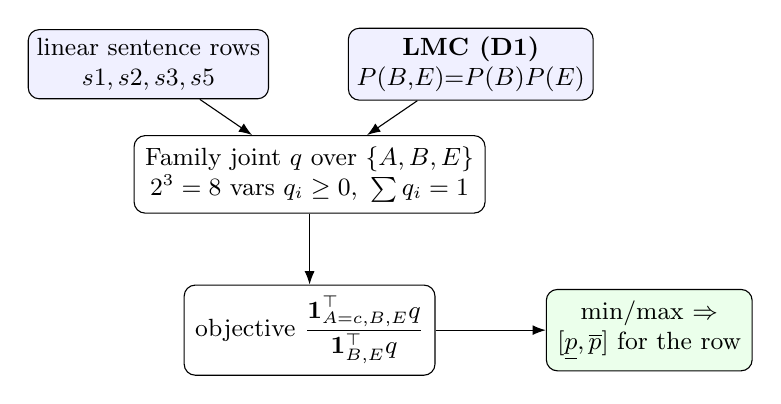
\begin{tikzpicture}[font=\small,>=Latex,node distance=6mm,
  box/.style={draw,rounded corners,inner sep=4pt,align=center},
  con/.style={draw,fill=blue!6,rounded corners,inner sep=3pt,align=center}]
  % top row: the constraint sources, well separated
  \node[con] (s) {linear sentence rows\\$s1,s2,s3,s5$};
  \node[con,right=10mm of s] (lmc) {\textbf{LMC (D1)}\\$P(B{,}E){=}P(B)P(E)$};
  % middle: the family joint, centred under the two sources
  \node[box,below=9mm of $(s)!0.5!(lmc)$] (joint)
    {Family joint $q$ over $\{A,B,E\}$\\$2^3=8$ vars $q_i\ge0,\ \sum q_i=1$};
  % bottom: objective then output
  \node[box,below=9mm of joint] (obj)
    {objective $\dfrac{\mathbf 1_{A=c,B,E}^\top q}{\mathbf 1_{B,E}^\top q}$};
  \node[box,fill=green!8,right=14mm of obj] (out)
    {min/max $\Rightarrow$\\$[\underline p,\overline p]$ for the row};
  \draw[->] (s) -- (joint);
  \draw[->] (lmc) -- (joint);
  \draw[->] (joint) -- (obj);
  \draw[->] (obj) -- (out);
\end{tikzpicture}
\caption{D1 (Algorithm~\ref{alg:d1}). The family-scope joint $q$ is constrained by the
  in-scope sentences \emph{and} the scope-restricted LMC equalities; the conditional bound is
  read off as a fractional objective. \texttt{"linear"} omits the blue LMC block.}
\label{fig:d1}
\end{figure}

% ======================================================================
\subsection{D2 --- scope merging with budget $k$ (\texttt{merge\_budget})}
\label{sec:d2-detail}

\paragraph{What it computes.} D2 is a \emph{pre-factorization} pass: before the local credal
sets are solved, it merges adjacent families into super-families whose flattened scope is at
most $k$ atoms, then runs D1 (or \texttt{"linear"}) on the larger scopes. Because a merged
scope is a superset of each member scope, more sentences and more LMC assertions become
in-scope, so the local sets can only tighten. At $k{=}1$ no merge happens (identical to
today); at $k\ge n$ everything collapses into one family (exact). D2 operates on a
\emph{copy} of \texttt{lcn.families} and never mutates the model.

\begin{algorithm}[t]
\caption{D2 family merging (\texttt{\_merge\_families})}
\label{alg:d2}
\begin{algorithmic}[1]
\Require families $\mathcal F=\{(\mathrm{ch}_i,\mathrm{pa}_i,S_i)\}$; budget $k$
\State build the \emph{family DAG}: a node per family child; an arc $u\!\to\!v$ whenever
  $\mathrm{ch}_u$ is a parent of $v$
\Repeat
  \ForAll{arcs $(u,v)$ in deterministic (sorted) order}
     \State $\mathrm{sc} \gets \mathrm{flatten}(\mathrm{scope}(u)\cup\mathrm{scope}(v))$
     \If{$|\mathrm{sc}| > k$} \textbf{continue} \EndIf
     \State form the super-family $M$: child atoms $=\mathrm{ch}_u\cup\mathrm{ch}_v$ (node name
       \texttt{"-".join(sorted(\dots))}); parents $=$ external parents only (drop parents
       produced inside $M$)
     \State rewire every family that had $u$ or $v$ as a parent to point at $M$
     \If{the rewired family DAG is acyclic} accept the contraction; \textbf{restart} the scan
     \Else{} reject (keep searching) \Comment{D2 never creates a cycle}
     \EndIf
  \EndFor
\Until{no contraction was accepted}
\ForAll{resulting (super-)families $M$}
  \State recompute attached sentences $S_M=\{s: \mathrm{atoms}(s)\subseteq\mathrm{scope}(M)\}$
    \Comment{can only grow}
\EndFor
\State \Return the merged family list (fed to D1/\texttt{"linear"} on the larger scopes)
\end{algorithmic}
\end{algorithm}

\paragraph{Worked example (\texttt{alarm}, $k{=}5$).} The families are $P(A\mid B,E)$ (scope
$\{A,B,E\}$), $P(B)$, $P(E)$, $P(C\!-\!D\mid A)$ (scope $\{C,D,A\}$). With $k{=}5$ the greedy
pass contracts the arc $A\!\to\!(C\!-\!D)$ (their union $\{A,B,E,C,D\}$ has size $5\le k$),
then folds $B$ and $E$ into the same super-family along the arcs $B\!\to\!A$, $E\!\to\!A$,
producing a single family over all five atoms (Figure~\ref{fig:d2}). Now \emph{every}
sentence and \emph{every} LMC assertion is in-scope, including the cross-family assertions
$(C\perp B,E\mid D,A)$ and $(D\perp B,E\mid C,A)$ that no $3$-atom family could host --- so the
$k{=}5$ local set is the exact joint and the $C\!-\!D$ conditionals tighten beyond what D1
achieves on the $3$-atom family. A budget $k{=}3$ would leave the families unchanged here
(every pairwise union already exceeds $3$), recovering plain D1.

\begin{figure}[t]
\centering
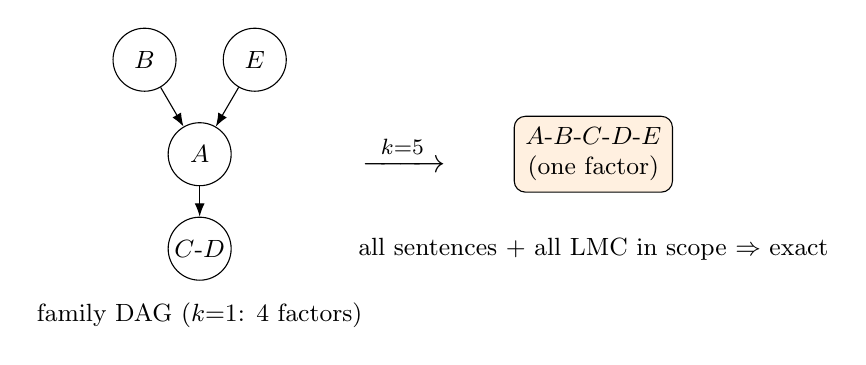
\begin{tikzpicture}[font=\small,>=Latex,
  fam/.style={draw,circle,minimum size=8mm,inner sep=1pt},
  sup/.style={draw,rounded corners,fill=orange!12,inner sep=4pt,align=center}]
  % left: family DAG
  \begin{scope}
    \node[fam] (B) at (0,0) {$B$};
    \node[fam] (E) at (1.4,0) {$E$};
    \node[fam] (A) at (0.7,-1.2) {$A$};
    \node[fam] (CD) at (0.7,-2.4) {$C{\text-}D$};
    \draw[->] (B) -- (A); \draw[->] (E) -- (A); \draw[->] (A) -- (CD);
    \node[below=0.15cm of CD] {family DAG ($k{=}1$: 4 factors)};
  \end{scope}
  % arrow
  \node at (3.3,-1.2) {\large $\xrightarrow{\ k=5\ }$};
  % right: merged
  \begin{scope}[xshift=5.0cm]
    \node[sup] (M) at (0.7,-1.2) {$A{\text-}B{\text-}C{\text-}D{\text-}E$\\(one factor)};
    \node[below=0.45cm of M] {all sentences + all LMC in scope $\Rightarrow$ exact};
  \end{scope}
\end{tikzpicture}
\caption{D2 (Algorithm~\ref{alg:d2}) on \texttt{alarm} with $k{=}5$: greedy arc contraction
  collapses the four families into one super-family over $\{A,B,C,D,E\}$, bringing the
  cross-family LMC assertions in-scope. At $k{=}1$ the left DAG is used unchanged.}
\label{fig:d2}
\end{figure}

% ======================================================================
\subsection{D3 --- certified local bounds (\texttt{solver="scip"})}
\label{sec:d3-detail}

\paragraph{What it computes.} D3 is not a separate model but a \emph{backend}: it solves the
D1 (or D2) local program with SCIP's spatial branch-and-bound global solver instead of the
local ipopt. The D1 program is nonconvex (Type-2 ratio constraints and the bilinear LMC
equalities), so ipopt only returns a \emph{locally} optimal bound, which can be strictly
looser \emph{or} (for a feasibility-style extreme) spuriously tighter than the true local
bound. SCIP returns the bound with a global optimality certificate (or a bounded gap under a
time limit). D3 thus serves two roles: it produces the exact local credal set $K_v^{\mathrm
{true}}$ for a family scope, and it \emph{certifies} the cheaper D1/ipopt bounds.

\begin{algorithm}[t]
\caption{D3 certified local bound (\texttt{solver="scip"} on the D1 model)}
\label{alg:d3}
\begin{algorithmic}[1]
\Require the D1 model $\mathcal M$ for (family, row, sense) from Algorithm~\ref{alg:d1}
\State add the denominator floor $\mathbf 1_p^\top q \ge \varepsilon$ (so the conditional ratio
  stays well defined and SCIP cannot drive $P(\mathrm{pa}{=}p)\!\to\!0$)
\State $(\text{val},\text{gap},\text{status}) \gets \textsc{ScipSolve}(\mathcal M,\
  \text{time\_limit},\ \text{gap\_tol})$
\If{$\text{status}\in\{\textsc{optimal}\}$ \textbf{or} $\text{gap}\le\text{gap\_tol}$}
  \Return certified $\text{val}$
\Else{} \Return best-so-far $\text{val}$ with the reported gap \Comment{partial certificate}
\EndIf
\end{algorithmic}
\end{algorithm}

\paragraph{Worked example (\texttt{alarm}, certifying $P(C\!-\!D\mid A)$).} On the diagonal
state $P(C{=}0,D{=}0\mid A{=}1)$ the isolated family LP gives $[0,0.7]$ (only the sum
$P(C{=}D\mid A)\le 0.7$ of $s4$ binds). Running the same model under \texttt{solver="scip"}
returns the identical interval \emph{with a zero optimality gap}, certifying that $0.7$ is the
true family-projected upper bound and that the ipopt result was not a local artifact. The
contract D3 enforces is the containment
\[
  [\,\underline p^\star,\ \overline p^\star\,]_{\text{D3/scip}} \;\subseteq\;
  [\,\underline p,\ \overline p\,]_{\text{D1/ipopt}} \;\subseteq\;
  [\,\underline p,\ \overline p\,]_{\text{linear}},
\]
checked per (family, row): a violation of the left inclusion flags an unsound ipopt local
optimum, the width gap on the right quantifies how much looseness D1 still leaves (gap~A
residual). Figure~\ref{fig:d3} shows the role.

\begin{figure}[t]
\centering
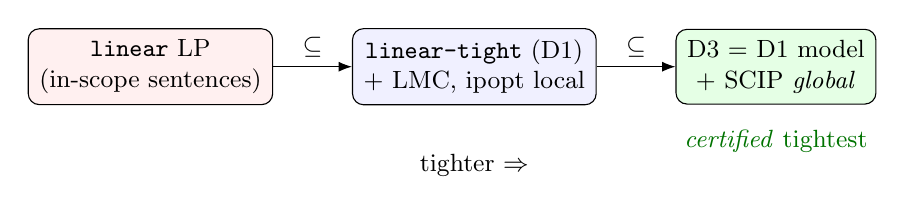
\begin{tikzpicture}[font=\small,>=Latex,
  b/.style={draw,rounded corners,inner sep=4pt,align=center}]
  \node[b,fill=red!6] (lin) {\texttt{linear} LP\\(in-scope sentences)};
  \node[b,fill=blue!6,right=1.0cm of lin] (d1) {\texttt{linear-tight} (D1)\\$+$ LMC, ipopt local};
  \node[b,fill=green!10,right=1.0cm of d1] (d3) {D3 = D1 model\\$+$ SCIP \emph{global}};
  \draw[->] (lin) -- node[above]{$\subseteq$} (d1);
  \draw[->] (d1) -- node[above]{$\subseteq$} (d3);
  \node[below=0.5cm of d1,align=center] {tighter $\Rightarrow$};
  \node[below=0.2cm of d3,align=center,text=green!45!black] {\emph{certified} tightest};
\end{tikzpicture}
\caption{D3 (Algorithm~\ref{alg:d3}) solves the D1 model with the global solver, certifying
  the local bound. The nesting $\text{D3}\subseteq\text{D1}\subseteq\texttt{linear}$ is the
  per-row validation contract (Section~\ref{sec:validation}).}
\label{fig:d3}
\end{figure}

% ======================================================================
\subsection{D4 --- region-restricted coupling (\texttt{coupling="cross-family"})}
\label{sec:d4-detail}

\paragraph{What it computes.} Credal VE represents each node's local credal set as a
\texttt{Potential}: a finite set of \emph{functions} (numpy arrays), each one a fully
instantiated CPT obtained by picking, independently per parent-configuration, one local
extreme point. Bucket elimination repeatedly \emph{combines} potentials (a Cartesian product
of their function sets) and \emph{marginalises} a variable out; the final query bound is the
$\min/\max$ of the normalised query state over the surviving functions. This is the free
strong-extension product. D4 \emph{drops} any function whose assembled joint violates a
\emph{cross-family} constraint --- a sentence or LMC assertion whose atom set is a subset of
no single family scope. Crucially, a fully assembled function over a node set \emph{is} the
unnormalised joint over those nodes' atoms, so a cross-family residual can be evaluated on it
directly, reusing exactly the verifier's residual math.

\paragraph{The two pieces that make it correct.}
\begin{enumerate}
  \item \textbf{Checkability gate.} A constraint is evaluated on a function only once the
    function's scope covers \emph{all} the constraint's atoms; until then the predicate
    returns ``feasible'' (do not drop). This makes filtering after \emph{any} elimination step
    sound: it can only ever remove a genuinely infeasible function, never one whose
    feasibility is undecided.
  \item \textbf{Order augmentation.} For the gate to ever fire, the constrained atoms must
    co-occur in some bucket. D4 therefore forces the min-fill elimination order, augmented
    with one extra ``clique scope'' per cross-family constraint (its node set), so those nodes
    land in a common bucket --- otherwise an atom is summed out before the constraint scope
    assembles and D4 stays inert (sound but useless).
\end{enumerate}

\begin{algorithm}[t]
\caption{D4 coupled Credal VE (\texttt{coupling="cross-family"})}
\label{alg:d4}
\begin{algorithmic}[1]
\Require credal net $\mathit{cnv}$; query $q$; evidence $e$
\State $\mathcal C \gets$ cross-family constraints
  $\{c:\mathrm{atoms}(c)\not\subseteq\mathrm{scope}(f)\ \forall\ \text{families } f\}$
\If{$\mathcal C=\varnothing$} run plain Credal VE \Comment{D4 inert; e.g.\ \texttt{alarm}}
\EndIf
\State $\mathit{order}\gets$ \textsc{MinFill}$\big(\text{factor scopes}\cup\{\,\text{node set
  of }c : c\in\mathcal C\},\ \text{exclude}{=}\{q\}\big)$
\State build one \texttt{Potential} per node from its extreme points; add evidence indicators
\ForAll{$v$ in $\mathit{order}$}
  \State $\mathit{bucket}\gets$ potentials whose scope contains $v$;
    $\mathit{combined}\gets$ product of the bucket
  \State \textbf{D4 filter:} keep $f\in\mathit{combined}$ iff
    $\textsc{Feasible}(f,\ \mathrm{scope}(\mathit{combined}),\ \mathcal C)$
    \Comment{on the full bucket scope, \emph{before} marginalising}
  \State $\mathit{result}\gets$ \textsc{Marginalise}$(\mathit{combined},v)$;
    $\mathit{result}\gets$ \textsc{Prune}$(\mathit{result})$
\EndFor
\State combine the leftovers; \Return $\min/\max$ of the normalised $q$ state over the
  surviving functions
\Statex
\Function{Feasible}{$f,\ \mathrm{sc},\ \mathcal C$}
  \ForAll{$c\in\mathcal C$ with $\mathrm{atoms}(c)\subseteq\mathrm{sc}$}
     \State marginalise $f$ to $\mathrm{atoms}(c)$, normalise, evaluate the residual
       (Type-1/2 bound or bilinear LMC); \textbf{if} violated \textbf{return} false
  \EndFor
  \State \Return true \Comment{atoms not yet all in scope $\Rightarrow$ not droppable}
\EndFunction
\end{algorithmic}
\end{algorithm}

\paragraph{Worked example (\texttt{d4\_biting}, query $P(B\mid C{=}1)$).} The cross-family
sentence is $P(B\land C)\le 0.05$ (atoms $\{B,C\}$, fitting neither the $B$ nor the $C$
family). The free product can pick $P(B{=}1\mid A)$ and $P(C{=}1\mid A)$ both large, giving a
joint with $P(B\land C)=0.92$ --- admissible in the strong extension but forbidden by the
LCN. Augmenting the order forces $\{A,B,C\}$ into one bucket; the D4 filter there drops every
function whose $P(B\land C)$ exceeds $0.05$. Figure~\ref{fig:d4} traces it. Net effect on the
\emph{unconditional} marginals is small, but on a query that makes $B$ and $C$ interact
(e.g.\ evidence $C{=}1$) the upper bound on $P(B\mid C{=}1)$ drops sharply.

\paragraph{A sharp limitation (conditional queries).} D4 is sound only as a tightening of the
strong-extension bound, and the strong-extension bound is itself a valid \emph{outer} bound
only for \emph{unconditional} marginals. For a conditional query $P(q\mid e)$ the bound is a
ratio whose extremum need not lie at a vertex of the unconditioned credal set, so
$\min/\max$-over-vertices --- and hence D4's filtered version --- can land \emph{strictly
inside} the true interval. On \texttt{d4\_biting}, $P(B\mid C{=}1)$ is truly $[0.006,0.926]$,
yet plain Credal VE reports $[0.038,0.963]$ and D4 the spurious near-point $[0.038,0.038]$.
The implementation prints a warning when \texttt{coupling="cross-family"} is used with
evidence and directs the user to D5 (Section~\ref{sec:d5-detail}), which is exact.

\begin{figure}[t]
\centering
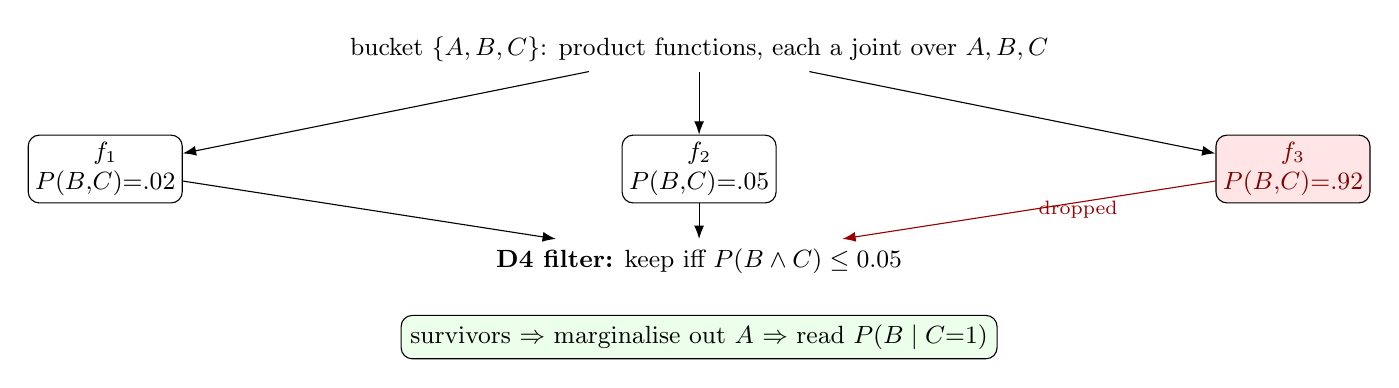
\begin{tikzpicture}[font=\small,>=Latex,
  fn/.style={draw,rounded corners,inner sep=2.5pt,align=center,minimum width=11mm},
  drop/.style={draw,rounded corners,inner sep=2.5pt,align=center,minimum width=11mm,
    fill=red!10,text=red!50!black}]
  \node[align=center] (lab) {bucket $\{A,B,C\}$: product functions, each a joint over $A,B,C$};
  \node[fn,below left=0.8cm and 2.0cm of lab] (f1) {$f_1$\\$P(B{,}C){=}.02$};
  \node[fn,below=0.8cm of lab] (f2) {$f_2$\\$P(B{,}C){=}.05$};
  \node[drop,below right=0.8cm and 2.0cm of lab] (f3) {$f_3$\\$P(B{,}C){=}.92$};
  \draw[->] (lab) -- (f1); \draw[->] (lab) -- (f2); \draw[->] (lab) -- (f3);
  \node[below=0.45cm of f2,align=center] (gate)
    {\textbf{D4 filter:} keep iff $P(B\land C)\le0.05$};
  \draw[->] (f1) -- (gate); \draw[->] (f2) -- (gate);
  \draw[->,red!60!black] (f3) -- node[right,font=\scriptsize]{dropped} (gate);
  \node[below=0.4cm of gate,draw,rounded corners,fill=green!8]
    {survivors $\Rightarrow$ marginalise out $A$ $\Rightarrow$ read $P(B\mid C{=}1)$};
\end{tikzpicture}
\caption{D4 (Algorithm~\ref{alg:d4}) on \texttt{d4\_biting}: in the augmented bucket
  $\{A,B,C\}$, functions whose joint violates the cross-family $P(B\land C)\le0.05$ (e.g.\
  $f_3$ with $0.92$) are dropped \emph{before} $A$ is summed out; the survivors yield the
  tightened query.}
\label{fig:d4}
\end{figure}

% ======================================================================
\subsection{D5 --- junction-tree exact NLP (\texttt{coupling="d5"})}
\label{sec:d5-detail}

\paragraph{What it computes.} D5 abandons the vertex product entirely and computes the
\emph{exact} chain-graph marginal by a single nonlinear program over \emph{cluster-marginal}
variables. Build a clique (junction) tree from the chain-graph elimination order; give each
cluster $c$ a variable vector $q_c$ ranging over the joint distribution of its atoms; tie
adjacent clusters with Lauritzen \emph{separator-consistency} equalities (the marginal of one
cluster onto a shared separator equals the neighbour's); and impose every LCN sentence and
LMC equality on a cluster whose atom set contains it. Reading the query marginal off the
cluster that holds the query (and evidence) and optimising it $\min/\max$ over this feasible
region returns the exact LCN bound. Because each cluster is bounded by the treewidth, the NLP
has $\sum_c 2^{|\mathrm{atoms}(c)|}$ variables rather than $2^n$.

\paragraph{Why it is exact.} For a chain graph the clique tree has the \emph{running
intersection property} (RIP). With RIP, a family of cluster marginals that (i) agrees on every
separator and (ii) satisfies, in some containing cluster, every LCN/LMC constraint, extends to
a single global joint feasible for the full $2^n$ \texttt{ExactInference} model --- and
conversely every feasible global joint projects to such a family. Hence the cluster NLP and
the full-joint NLP have the same optimal value. Cross-family constraints (and the
query$+$evidence atoms) are forced to share a host cluster by augmenting the elimination order
with their node sets, exactly as in D4; if that would push a cluster past the treewidth
budget, D5 falls back to \texttt{ExactInference.run\_query} (still exact, at $2^n$).

\begin{algorithm}[t]
\caption{D5 junction-tree exact NLP (\texttt{build\_and\_solve\_jt\_nlp})}
\label{alg:d5}
\begin{algorithmic}[1]
\Require credal net $\mathit{cnv}$; query $q$; evidence $e$; budget $k_{\max}$; solver
\State $\mathcal C\gets$ cross-family constraints; augment the min-fill order with their node
  sets and the query$+$evidence node set
\State build the clique tree $T$ (clusters $\mathcal K$, edges with separators) from the
  augmented order; flatten each cluster to its atom set; prune leaf clusters subsumed by a
  neighbour
\If{$\max_{c}|\mathrm{atoms}(c)| > k_{\max}$} \Return \textsc{ExactInference}$(q,e)$
  \Comment{budget fallback}
\EndIf
\State create variables $q_c[i]\ge 0$ for each cluster $c$ and state $i\in[0,2^{|\mathrm
  {atoms}(c)|})$; add per-cluster simplex $\sum_i q_c[i]=1$
\ForAll{tree edges $(c,d)$ with separator $S$}
  \State build $0/1$ marginalisation matrices $M_{c\to S},M_{d\to S}$;
    add $M_{c\to S}\,q_c = M_{d\to S}\,q_d$ \Comment{separator consistency}
\EndFor
\ForAll{sentences / LMC assertions} assign each to a host cluster containing its atoms; add
  its row(s) (Type-1/2 linear/ratio, or bilinear LMC) on that cluster's $q_c$
\EndFor
\State on the host cluster $c_q$ of $q{\cup}e$, build the objective
  $P(q{=}1\mid e)=(\mathbf 1_{q,e}^\top q_{c_q})/(\mathbf 1_{e}^\top q_{c_q})$
  via the aux-variable trick (with denominator floor under SCIP)
\State $\underline q\gets \textsc{Solve}(\min)$, $\overline q\gets \textsc{Solve}(\max)$ with
  the global backend (SCIP); \Return $[\underline q,\overline q]$
\end{algorithmic}
\end{algorithm}

\paragraph{Worked example (\texttt{d4\_biting}, query $P(B\mid C{=}1)$).} The cross-family
sentence $P(B\land C)\le 0.05$ has node set $\{B,C\}$, and the query$+$evidence atoms are
$\{B,C\}$; augmenting forces them together, so the elimination yields a clique tree with a
cluster $c_q{=}\{A,B,C\}$ (the full joint) and a subsumed leaf that is pruned. All four
sentences, the LMC assertion $(B\perp C\mid A)$, and the objective all host on $c_q$. The NLP
is therefore identical to the full-joint \texttt{ExactInference} model, and solving it with
SCIP returns $P(B\mid C{=}1)=[0.006,0.926]$ --- the exact bound, matching the certified global
oracle and correcting both plain Credal VE ($[0.038,0.963]$) and D4 ($[0.038,0.038]$).
Figure~\ref{fig:d5} shows the cluster tree and the NLP it induces.

\paragraph{Two implementation findings.} (1)~The cluster NLP is nonconvex (Type-2 ratios,
bilinear LMC, the conditional-ratio objective); the local solver ipopt returns a local
optimum that can fall \emph{short} of the bound (it gave $0.90$ instead of $0.926$ above), so
D5 defaults to the certified global backend SCIP. (2)~The treewidth saving is real only when
the cross-family constraints are themselves local: on \texttt{alarm} the assertions $(C\perp
B,E\mid D,A)$ and $(D\perp B,E\mid C,A)$ span all five atoms, so the augmentation forces a
near-full-joint cluster and D5 degenerates to \texttt{ExactInference} cost there.

\begin{figure}[t]
\centering
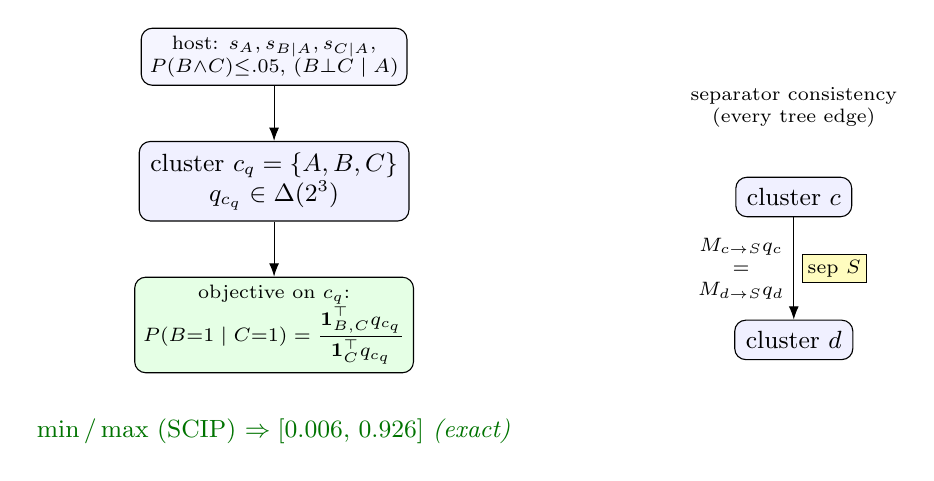
\begin{tikzpicture}[font=\small,>=Latex,
  cl/.style={draw,rounded corners,inner sep=4pt,align=center,fill=blue!6},
  sep/.style={draw,rectangle,inner sep=2pt,fill=yellow!25,font=\scriptsize},
  con/.style={draw,rounded corners,inner sep=3pt,fill=blue!4,font=\scriptsize,align=center}]
  % cluster tree (left)
  \node[cl] (cq) {cluster $c_q=\{A,B,C\}$\\$q_{c_q}\in\Delta(2^3)$};
  \node[con,above=0.7cm of cq] (rows)
    {host: $s_{A},s_{B|A},s_{C|A}$,\\ $P(B{\land}C){\le}.05$, $(B{\perp}C\mid A)$};
  \draw[->] (rows) -- (cq);
  % objective
  \node[con,below=0.7cm of cq,fill=green!10] (obj)
    {objective on $c_q$:\\$P(B{=}1\mid C{=}1)=\dfrac{\mathbf 1_{B,C}^\top q_{c_q}}{\mathbf 1_{C}^\top q_{c_q}}$};
  \draw[->] (cq) -- (obj);
  \node[below=0.45cm of obj,align=center,text=green!45!black]
    {$\min/\max$ (SCIP) $\Rightarrow [0.006,\,0.926]$ \emph{(exact)}};
  % a generic edge illustration (right)
  \begin{scope}[xshift=6.6cm,yshift=-0.2cm]
    \node[cl] (c1) {cluster $c$};
    \node[cl,below=1.3cm of c1] (c2) {cluster $d$};
    \node[sep,right=0.1cm of $(c1)!0.5!(c2)$] (s) {sep $S$};
    \draw[->] (c1) -- node[left,font=\scriptsize,align=center]{$M_{c\to S}q_c$\\$=$\\$M_{d\to S}q_d$} (c2);
    \node[above=0.5cm of c1,align=center,font=\scriptsize]
      {separator consistency\\(every tree edge)};
  \end{scope}
\end{tikzpicture}
\caption{D5 (Algorithm~\ref{alg:d5}) on \texttt{d4\_biting}: the augmented clique tree has the
  full-joint cluster $c_q=\{A,B,C\}$ hosting all constraints and the conditional objective;
  separator-consistency equalities (right) tie clusters on general instances. Solving with
  SCIP gives the exact $P(B\mid C{=}1)$.}
\label{fig:d5}
\end{figure}

The \texttt{cn/} package ships five inference algorithms beyond CVE. Crucially, \emph{all of
them consume the same object}: a built \texttt{CredalNetworkVertices}, i.e.\ the directed
structure plus the enumerated extreme points of the local credal sets
(\texttt{cnv.extreme\_points}). They differ only in how they propagate those vertices:

\begin{center}
\begin{tabular}{lll}
  \toprule
  Algorithm & Propagation & Bound character vs.\ the strong extension \\
  \midrule
  Credal VE (\texttt{cve.py})    & bucket elimination          & exact (the strong-extension interval) \\
  Credal CTE (\texttt{ccte.py})  & two-pass bucket tree        & exact ($\epsilon{=}0$); outer if $\epsilon{>}0$ \\
  ApproxLP (\texttt{approxlp.py})& per-variable LP over vertices & \emph{inner} (subset of the true interval) \\
  Interval BP (\texttt{ibp.py})  & loopy interval messages     & \emph{outer} (\texttt{interval}); inner (\texttt{variational}) \\
  Credal IJGP (\texttt{ijgp.py})  & join-graph, $i$-bound       & outer-style; tunable by $i$-bound \\
  \bottomrule
\end{tabular}
\end{center}

The essential observation is that every one of these algorithms brackets the
\emph{strong-extension} interval $[\underline{q}_{\mathrm{SE}},\overline{q}_{\mathrm{SE}}]$,
not the LCN interval $[\underline{q}_{\mathrm{LCN}},\overline{q}_{\mathrm{LCN}}]$. Since
\[
  [\underline{q}_{\mathrm{LCN}},\overline{q}_{\mathrm{LCN}}]
  \;\subseteq\;
  [\underline{q}_{\mathrm{SE}},\overline{q}_{\mathrm{SE}}],
\]
shrinking the strong extension toward $\mathcal{D}_{\mathrm{LCN}}$ pulls every algorithm's
output inward. This splits the schemes into two leverage classes.

\paragraph{Class 1 --- input-level tightening (D1, D2, D3): free for all five algorithms.}
D1/D2/D3 change only what \texttt{CredalNetworkVertices.from\_lcn} produces---tighter local
intervals, hence tighter enumerated vertices. Because the algorithms read those vertices
without assuming how they were obtained, \emph{no algorithm code changes}. The effects
compose with each algorithm's own character:
\begin{itemize}
  \item \textbf{CVE / CCTE} (exact over the strong extension): their interval is exactly
    $[\underline{q}_{\mathrm{SE}},\overline{q}_{\mathrm{SE}}]$, so a tighter strong
    extension is reported verbatim---the cleanest beneficiary.
  \item \textbf{ApproxLP} (inner): its interval sits \emph{inside} the strong-extension
    interval. Tighter vertices raise its lower bound and lower its upper bound too, but the
    inner gap remains; pairing ApproxLP (inner) with CVE (outer) on the \emph{same} tightened
    vertices brackets the LCN truth from both sides.
  \item \textbf{Interval BP} (outer): tighter local messages mean tighter fixed-point
    intervals; the loopy outer slack is unchanged but starts from a narrower base.
  \item \textbf{IJGP}: tighter cluster potentials propagate through the join graph; the
    $i$-bound still trades cost for tightness independently.
\end{itemize}
On the example, replacing the vacuous $[0,1]$ rows (D1) with genuine sub-intervals narrows
the vertex sets fed to \emph{all five}, so e.g.\ a query $P(A)$ tightens for CVE, ApproxLP,
IBP, CTE and IJGP simultaneously, with one build-stage change.

\paragraph{Class 2 --- propagation-level coupling (D4, D5): per-algorithm work.}
D4/D5 do not merely narrow intervals; they remove vertex \emph{combinations} (D4) or avoid
forming the product altogether (D5). This is a change to the propagation, so each algorithm
needs its own adaptation:
\begin{itemize}
  \item \textbf{CVE / CCTE}: add the cross-vertex side constraints (D4) to the bucket /
    cluster combination step. This is the most natural fit---both already optimize over
    vertex tuples per bucket, so a coupling constraint slots in directly. D5 is essentially
    a constraint-aware rewrite of CVE's bucket optimization.
  \item \textbf{ApproxLP}: its per-variable LP already optimizes over a vertex polytope;
    D4's coupling constraints can be added as extra LP rows, keeping the inner-bound
    guarantee while shrinking the polytope.
  \item \textbf{Interval BP / IJGP}: message passing does not carry global cross-factor
    constraints naturally. The practical route is to let D4's coupling be absorbed at the
    \emph{build} stage where possible (so it reduces to Class 1 for these two), and accept
    that the residual coupling D4 cannot localize is simply not captured by loopy / join-graph
    propagation---these remain the loosest of the family, by design.
\end{itemize}

\paragraph{Practical recommendation.}
Because Class 1 is free for all algorithms, apply D1 (and D2 where affordable) at the build
stage \emph{first}; every downstream algorithm benefits without modification. Reserve the
per-algorithm D4/D5 work for CVE/CCTE (and ApproxLP), which can absorb the coupling exactly,
and treat IBP/IJGP as fast outer approximations that ride on the Class-1 tightening.

\section{Validation strategy}\label{sec:validation}

Tightening must be checked against ground truth on two fronts, matching the two gaps.

\paragraph{Local-set tightness (gap A) via D3.}
D3 is itself the certifier: for any candidate local credal set produced by D1 or D2,
compare its interval $[\underline{p},\overline{p}]$ for each (family, interpretation)
against the D3 certified-global interval $[\underline{p}^\star,\overline{p}^\star]$
obtained from the SCIP joint-LP. A correct outer approximation requires
$[\underline{p}^\star,\overline{p}^\star]\subseteq[\underline{p},\overline{p}]$, and the
width difference quantifies the residual local looseness D1/D2 leave behind. Because D3
uses the global \texttt{solver="scip"} path, these reference intervals are certified, not
merely local optima---unlike \texttt{ExactInference}, which is only a local solver and is
not a reliable oracle.

\paragraph{Extension tightness (gap B) via \texttt{verify\_lmc\_factorization.py}.}
The factorization verifier reconstructs each product joint from a choice of local extreme
points and evaluates the LMC residual
\[
  P(x,y,s)\,P(s) - P(x,s)\,P(y,s) \;\approx\; 0
\]
for every assertion (its \texttt{lmc\_constraint\_groups\_vec} residuals). A residual that
stays $\le\texttt{tol}$ after a tightening change confirms the scheme has not broken the
independence structure while shrinking the set; a non-trivial residual that the LCN does
\emph{not} permit localizes a strong-extension (gap B) violation that D4/D5 must address.
This check is solver-free and deterministic, so it is a stable regression gate.

\paragraph{End-to-end.}
On small instances, posterior marginals from CVE under each scheme are compared to the
D3-style full-joint bounds for the query atom (the same certified global solve, with the
query as objective). The recommended sequence is D1, then D2 with D3 as the per-instance
certifier of gap A; D4/D5 are pursued only once the D3 comparison shows the residual gap is
genuinely the strong-extension gap B rather than remaining local looseness.

\end{document}
